\documentclass{article}

\title{ECO206 Microeconomic Theory Summary I}
\author{Tianyu Du}
\date{\today}

\usepackage{amsmath}
\usepackage{amssymb}
\usepackage{graphicx}
\usepackage{float}
\usepackage{mycommands}

\newcommand{\mc}[1]{\mathcal{#1}}

\begin{document}
	\maketitle
	\tableofcontents
	
	\section{Lecture 1 Introduction}
		\paragraph{Notation} Assuming there are $n$ goods, then a \textbf{bundle} of goods, $\mathcal{A}$ can be denoted as
		\[
			\sset{x^A}{1}{n} \in \R^n_{+}
		\]
		
		\subsection{Types of Income and Budget Set}
			Let $\vec{p} \in \R^n$ denote the \textbf{price vector}.
			\paragraph{Exogenous income} Let $I \in \R_+$ denote the \textbf{exogenous income}, then the budget set can be expressed as
			\[
				\mathcal{B} = \{\vec{x} \in \R^n_+ \ | \ \vec{x} \cdot \vec{p} \leq I \}
			\]
			
			\paragraph{Endogenous income} Let $\vec{\omega} \in \R^n_+$ denote the \textbf{endowment} and the budget set can be expressed as
			\[
				\mathcal{B} = \{\vec{x} \in \R^n_+ \ | \ \vec{x} \cdot \vec{p} \leq \vec{\omega} \cdot \vec{p}\}
			\]
		
		\subsection{Opportunity Cost}
			\paragraph{MRT} Marginal Rate of Transformation (MRT) measures, given budget constraint, the unit of a good need to be given up in order to consume one additional unit of the other good. \underbar{\emph{OC/MRT is expressed in units of a good, instead of dollar.}}
			\begin{multline*}
				\emph{Mathemtically, }\\
				\tx{Two-goods example, } \\
				E = x_1 p_1 + x_2 p_2 = y \\
				\tx{Take total differential, }\\
				dy = \pd{E}{x_1} dx_1 + \pd{E}{x_2} dx_2 = 0\\
				\implies \diff{x_2}{x_1} = -\frac{p_1}{p_2} \\
				\blacksquare
			\end{multline*}
			\paragraph{Interpretation} Units of good $x_2$ to given up (negative sign) in exchange for one unit of $x_1$.
	
		\subsection{Comparative Statics}
			\subsubsection{Pure Income Effect}
			\begin{figure}[h]
				\centering
				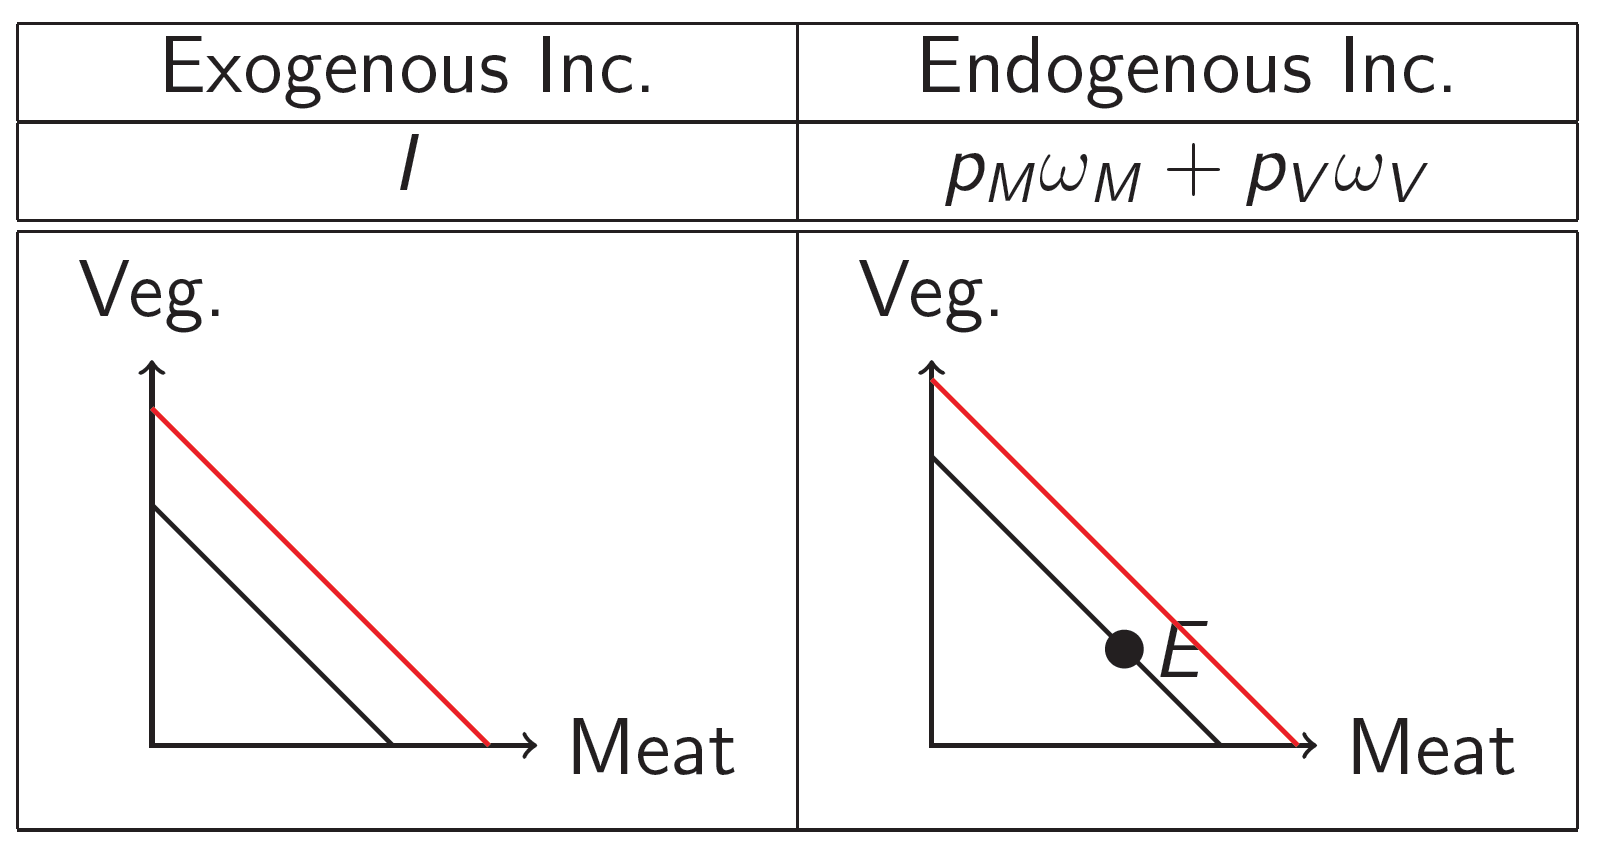
\includegraphics[width=0.8\linewidth]{figure/lec1_1}
				\caption{pure income effect from increase in income}
			\end{figure}
			\emph{For both types of income, pure income effect shifts the budget line parallel.}
			\newpage
			\subsubsection{Price Changes}
				\paragraph{Exogenous income} Consider a price increase in meat, in this case, the \emph{invariant bundle} (i.e. the bundle that is not affected by the price change at all) is on y-intercept.
				\begin{figure}[h]
					\centering
					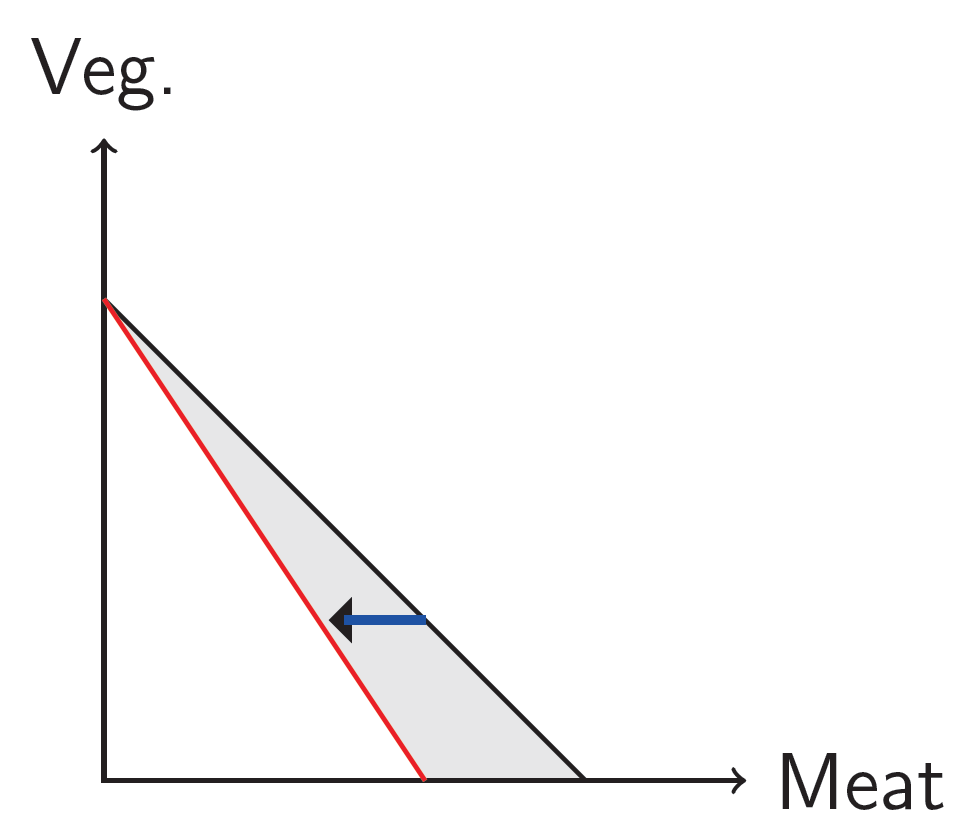
\includegraphics[width=0.5\linewidth]{figure/lec1_2}
					\caption{increase in price of meat on exogenous income budget line}
				\end{figure}
				
				\paragraph{Endogenous income} in this case, the \emph{invariant bundle} is the endowment bundle.
				\begin{figure}[h]
					\centering
					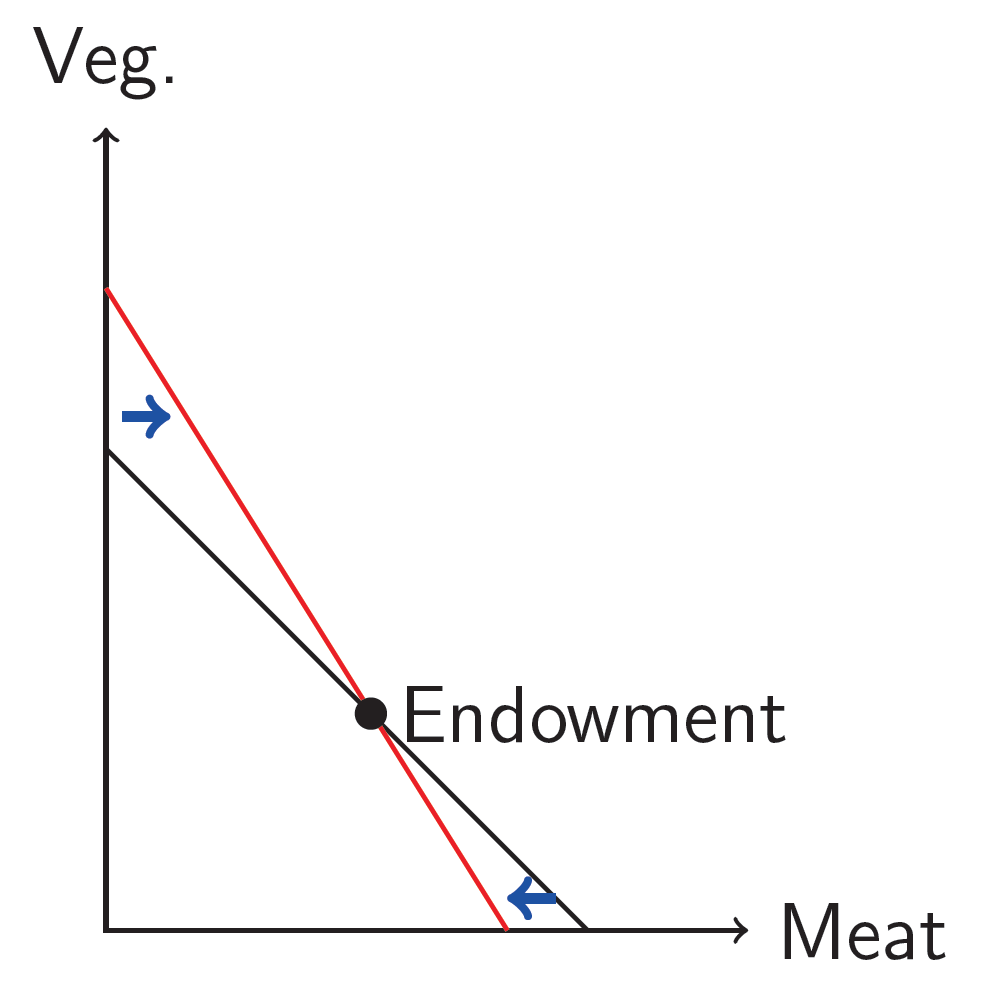
\includegraphics[width=0.5\linewidth]{figure/lec1_3}
					\caption{increase in price of meat on endogenous income budeget line}
				\end{figure}
				\paragraph{Note} In both cases, price change causes the budget line rotates around the invariant bundle.
				
				
	\section{Lecture 2 Preference and Utility}
		\subsection{Preference Relation}
			\emph{Preference Relation is Binary.}
			Let $\mc{X}$ be the consumption set, and let $\mc{A}, \mc{B} \in \mc{X}$.
			\paragraph{Definition} If a bundle $\mathcal{A}$ is no worse than (i.e. \textbf{at least as good as}) another bundle $\mathcal{B}$, then we denote this as
				\[
					\mathcal{A} \succcurlyeq \mathcal{B}
				\]
			\paragraph{Definition} A consumer \textbf{strictly prefers} bundle $\mathcal{A}$ than bundle $\mathcal{B}$ if and only if 
				\[
					\mc{A} \succcurlyeq \mc{B} \land \neg \mc{B} \succcurlyeq \mc{A}
				\]
				and denoted as
				\[
					\mc{A} \succ \mc{B}
				\]
			\paragraph{Definition} A consumer is \textbf{indifferent} between two bundles $\mc{A}$ and $\mc{B}$ if and only if
				\[
					\mc{A} \succcurlyeq \mc{B} \land \mc{B} \succcurlyeq \mc{A}
				\]
		
		\subsection{Rationality Assumptions}
			Let $\mc{X}$ denote the consumption set.
			\paragraph{A1.Completeness} A preference relation $\succcurlyeq$ is \textbf{complete} if and only if
				\[
					\mc{A} \succcurlyeq \mc{B} \lor \mc{B} \succcurlyeq \mc{A},\ \forall \mc{A},\mc{B} \in \mc{X}
				\]
			\paragraph{A2.Transitivity} A preference relation $\succcurlyeq$ is \textbf{transitive} if and only if
				\[
					\mc{A} \succcurlyeq \mc{B} \land \mc{B} \succcurlyeq \mc{C} \implies \mc{A} \succcurlyeq \mc{C},\ \forall \mc{A},\mc{B},\mc{C} \in \mc{X}
				\]
			\paragraph{Definition} a preference relation is \textbf{rational} if and only if it satisfies assumptions A1 and A2 above.
			
		\subsection{Convenience Assumptions}
			\paragraph{A3.Monotonicity} Let $\mc{A} = \sset{x^A}{1}{n}$ and $\mc{B} = \sset{x^B}{1}{n} \in \mc{X}$, then 
			\[
				x^A_i \geq x^B_i,\ \forall i \in \{1,\dots,n\} \implies \mc{A} \succcurlyeq \mc{B}
			\]
			and 
			\[
				x^A_i > x^B_i,\ \forall i \in \{1,\dots,n\} \implies \mc{A} \succ \mc{B}		
			\]
			\textbf{Example} In figure below, region 3 (including boundary) represents the \emph{no worse than set} of $\mc{A}$, i.e. $R_3 = \ \succcurlyeq(\mc{A}) := \{\vec{x} \in \mc{X}\ |\ \vec{x} \succcurlyeq \mc{A}\}$ and region 2 (including boundary) represents the \emph{no better than set} of $\mc{A}$, i.e. $R_2 = \succcurlyeq(\mc{A}) := \{\vec{x} \in \mc{X}\ | \ \mc{A} \succcurlyeq \vec{x}\} $
			\begin{figure}[h]
				\centering
				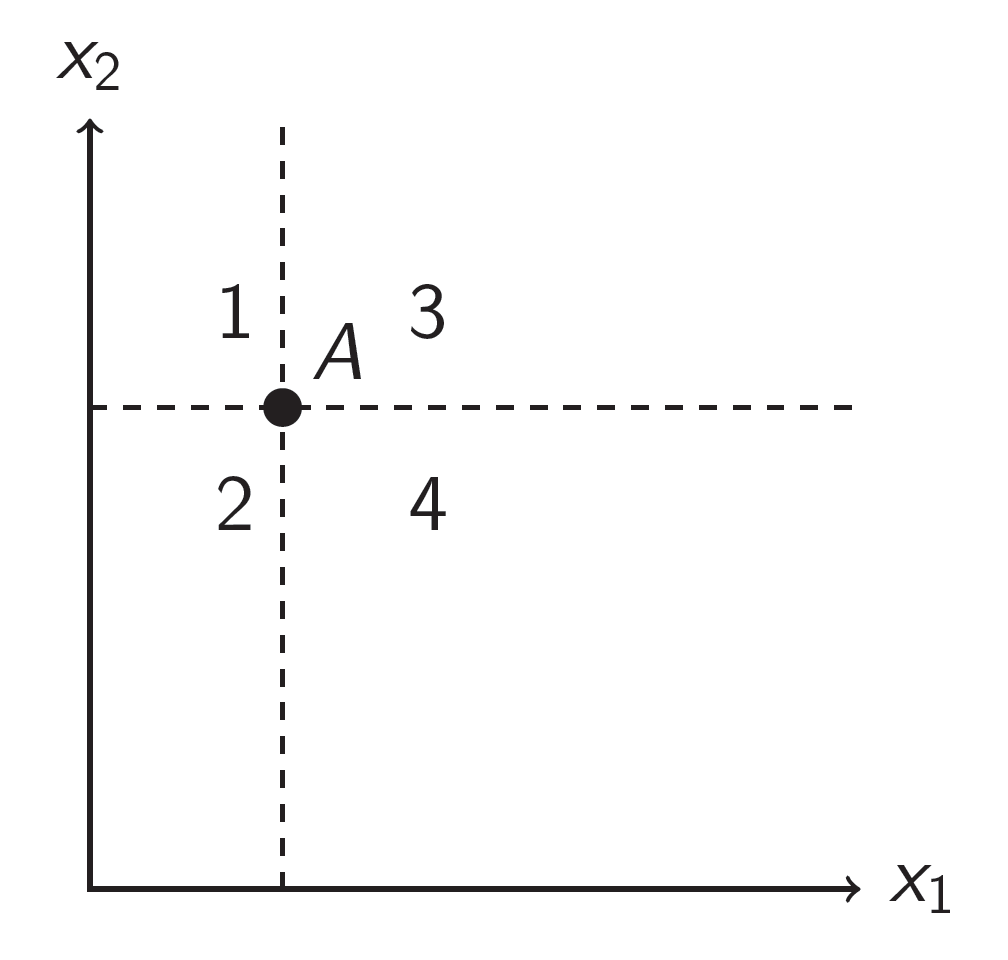
\includegraphics[width=0.5\linewidth ]{figure/lec2_1}
				\caption{monotonic preference}
			\end{figure}
			
			\paragraph{A4.(Weak) Convexity} If a preference relation is \textbf{convex}, then, for any $\mc{A}, \mc{B} \in \mc{X}$, suppose $\mc{A} \sim \mc{B}$,
			\[
				\alpha \mc{A} + (1-\alpha) \mc{B} \succcurlyeq \mc{A},\ \forall \alpha \in [0,1]
			\]
			\textbf{Meaning} the \emph{no worse than set} for any given bundle $\mc{A}$ over preference relation $\succcurlyeq$ is a convex set.
			\newline 
			\textbf{Implication} the utility function has to be quasi-concave.
			\newline
			\textbf{Lemma} the upper level contour for a quasi-concave function is convex.
			\paragraph{A5.Continuity} Loosely speaking, no sudden switch over preference. Formally, $\succcurlyeq(\mc{A})$ and $\preccurlyeq(\mc{A})$ sets are closed.
		
		\subsection{Indifference Curve}
			\paragraph{Definition} Let $\mc{A} \in \mc{X}$, then indifference set of $\mc{A}$ over preference relation $\succcurlyeq$ is defined as
			\[
				\sim(\mc{A}) = \{\vec{x} \in \mc{X}\ | \ \vec{x} \sim \mc{A}\}
			\]
			
		\subsection{Utility Function}
			\paragraph{Definition} a real-valued function $\trans{u}{\R^n_+}{\R}$ represents a preference relation if and only if, let $\vec{x_1}, \vec{x_2} \in \R^n_+$ denote the quantities of goods in bundles $\mc{A}_1$ and $\mc{A}_2 \in \mc{X}$,
			\[
				\mc{A}_1 \succcurlyeq \mc{A}_2 \iff u(\vec{x_1}) \geq u(\vec{x_2})
			\]
			
			\paragraph{Theorem} an utility function is invariant to \underbar{positive-monotonic} transformations. That's, let $g$ denote a positive-monotonic transformation, and $\trans{u}{\R^n_+}{\R}$ be a utility function representing preference relation $\succcurlyeq$, then $g\circ u$ also is an utility function representing $\succcurlyeq$.
			
			\paragraph{Definition} we say two consumers have the \textbf{same tastes} if and only if (1) they have same willingness to trade (MRS) at the same bundle \underbar{and} (2) same direction of increasing preference. 
			\newline Mathematically,
			\[
				MRS_1|_{\vec{x}} = MRS_2 | _{\vec{x}},\ \forall \vec{x} \in \mc{X}
			\] and, let $u_1$ and $u_2$ denote utility functions, then 
			\[
				\nabla u_1 \cdot \vec{d} \geq 0 \iff \nabla u_2 \cdot \vec{d} \geq 0,\ \forall \ \vec{d} \in \R^n
			\]
		
		\subsection{Marginal Rate of Substitution}
			\paragraph{Definition} MRS represents the \underbar{willingness to trade}. In two-goods situations, it measures the number of goods 2 the consumer is willing to give up for one unit of good 1, keeping his/her utility level constant.
			\begin{multline*}
				\emph{Mathematically, } \\
				du(\cdot) = \pd{u}{x_1}dx_1 + \pd{u}{x_2}dx_2 = 0\\
				\implies \diff{x_2}{x_1} = - \frac{\pd{u}{x_1}}{\pd{u}{x_2}} = - \frac{MU_1}{MU_2} \\
				\blacksquare
			\end{multline*}
		
		\subsection{Types of Preference Relations}
			\paragraph{Definition} A preference relation is homothetic if and only if there exists a homogeneous utility function to represent it. That's
			\[
				u(\alpha \vec{x}) = \alpha^k u(\vec{x})\ \tx{for some } k \in \mathbb{Z}^+\ \forall \alpha \in \R_+,\ \vec{x} \in \R^n_+
			\]
			Note that, utility function is invariant to positive monotonic transformation.
			
			\paragraph{Proposition} MRS of a homothetic preference only depends on the ratio of consumption. i.e. $MRS_{homothetic} = f(\frac{x_2}{x_1})$.
			
			\begin{figure}[h]
				\centering
				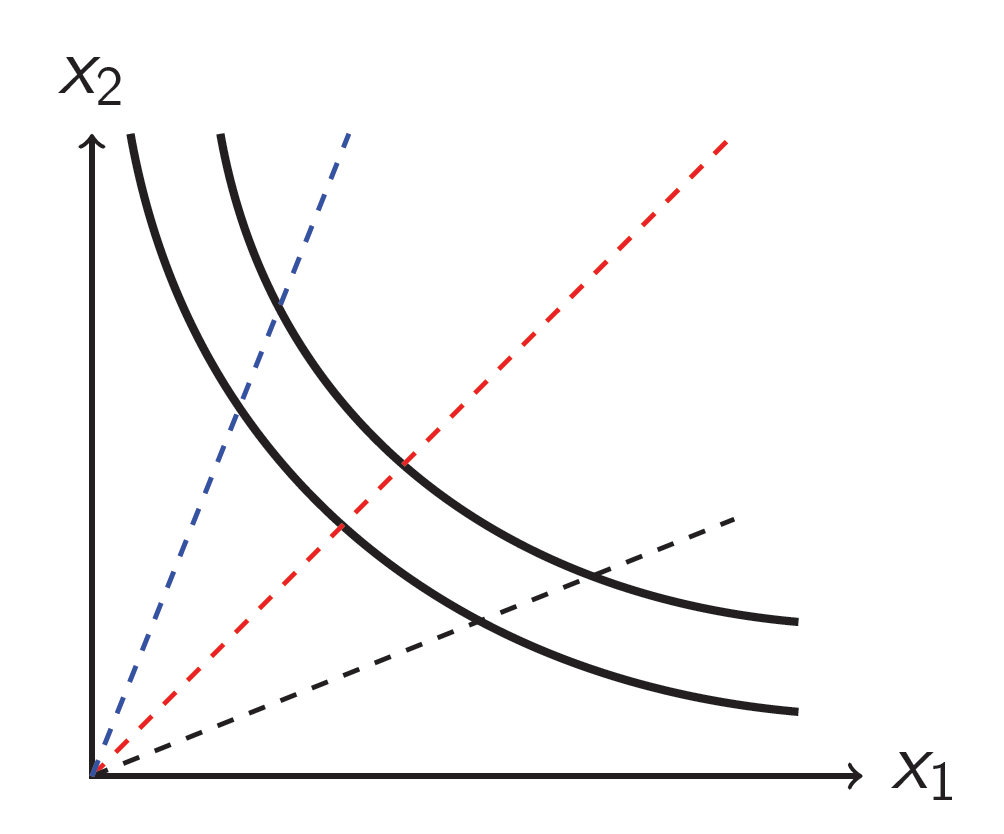
\includegraphics[width=0.35\linewidth]{figure/lec2_2}
				\caption{homothetic preference and MRS of it}
			\end{figure}
			
			\paragraph{Definition} A preference relation is \textbf{quasi-linear} in good $i$ if and only if, for all $\mc{A}$ and $\mc{B} \in \mc{X}$, 
			\[
				\mc{A} \sim \mc{B} \implies (\mc{A} + \alpha \vec{e_i}) \sim (\mc{B} + \alpha \vec{e_i}),\ \forall a \in \R
			\] where $\vec{e_i}$ is the $i^{th}$ standard basis vector of $\R^n$.
			
			\paragraph{Proposition} MRS of a quasi-linear utility depends only on one goods.
			
			\begin{figure}[h]
				\centering
				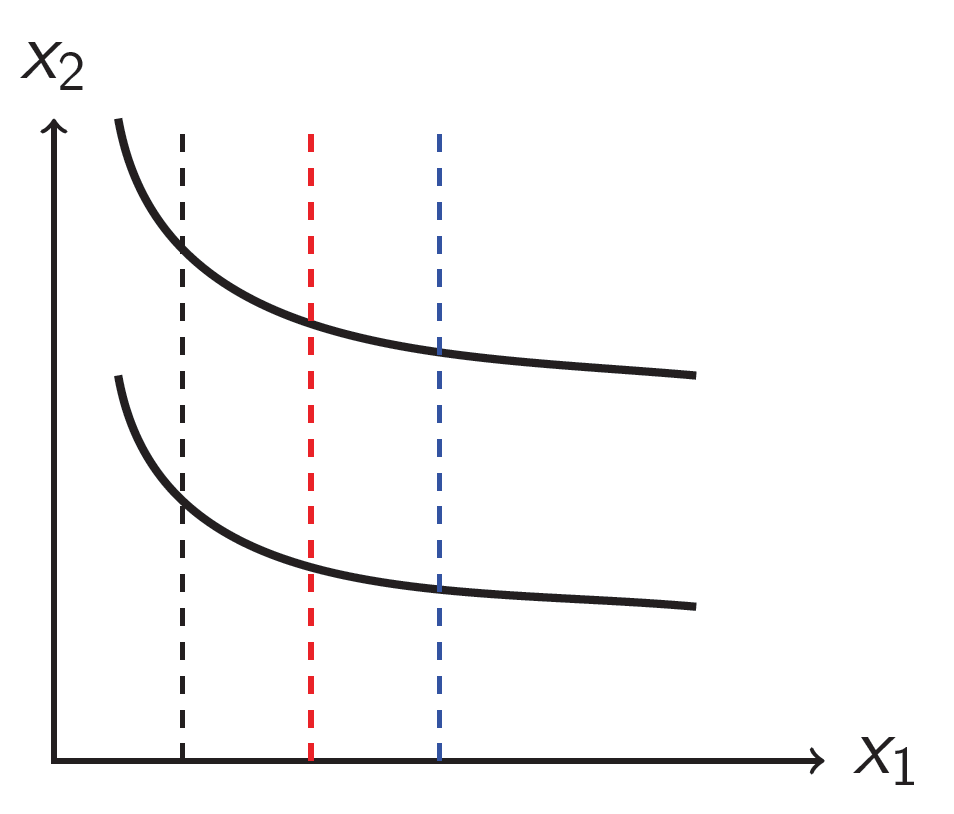
\includegraphics[width=0.35\linewidth]{figure/lec2_3}
				\caption{quasi-linear preference and MRS of it}
			\end{figure}
			 
	\section{Lecture 3 Choice}
		\subsection{Different Types of Tastes}
			\paragraph{Examine} 
				\begin{enumerate}
					\item How MRS changes \textbf{along} an IC.
					\item How MRS changes as we move \textbf{across} ICs.
				\end{enumerate}
		
		\subsection{Shape and Substitutability Along a given IC}
			\begin{figure}[h]
				\centering
				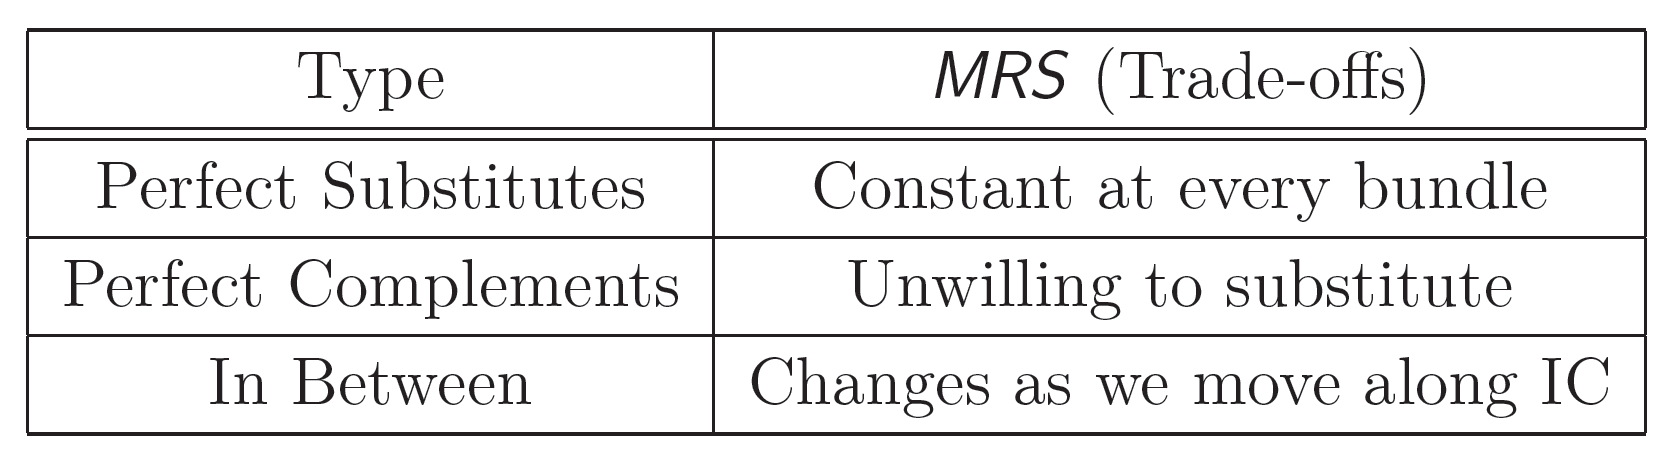
\includegraphics[width=0.7\linewidth]{figure/lec3_1}
				\caption{different types of preference and substituability}
			\end{figure}
		
			\begin{figure}[h]
				\centering
				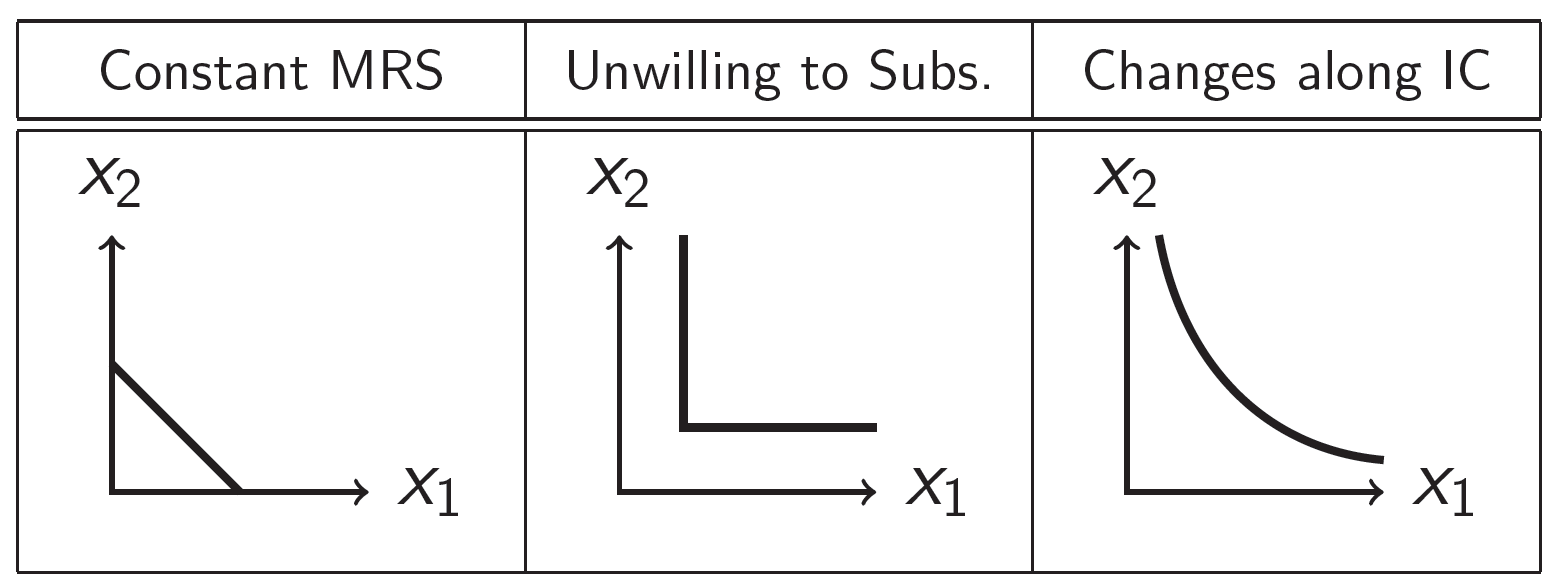
\includegraphics[width=0.7\linewidth]{figure/lec3_2}
				\caption{different types of preference and graphs}
			\end{figure}
		
		\subsection{Diminishing MRS}
			\paragraph{Definition} When we move down (more $x$ and less $y$) along an indifference curve.
			\begin{figure}[h]
				\centering
				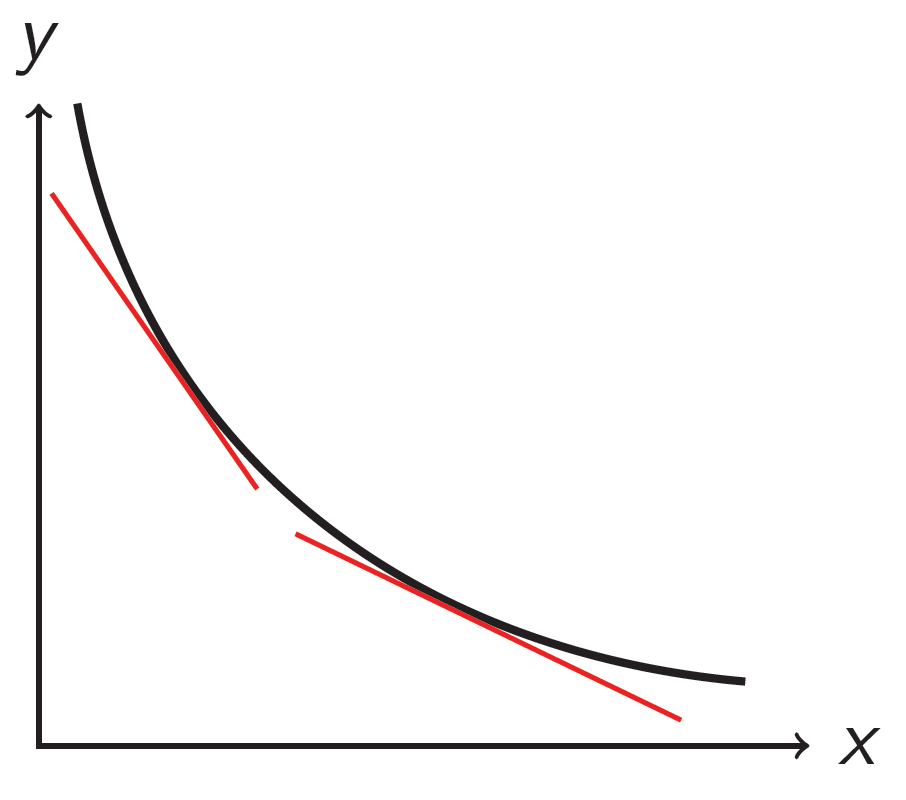
\includegraphics[width=0.5\linewidth]{figure/lec3_3}
				\caption{diminishing in MRS on graph}
			\end{figure}
			
			\paragraph{Diminishing MRS in words} Compare two bundles on the \emph{same} indifference curve. At each bundle consider how much of $y$ this consumer are willing to give up for an additional unit of $x$. Diminishing means if we have relative \emph{more} $x$ in one bundle, then we are \emph{less} willing to give up $y$ at that bundle compared to the other bundle.
			
			\paragraph{Note} Perfect substitution preference is linear and therefore quasi-linear.
			
		\subsection{Choice}
			\subsubsection{Tangency}
				\paragraph{MRS} units of $x_2$ that we are \textbf{willing} to pay for 1 more unit of $x_1$.
				\paragraph{Opp. Cost} units of $x_2$ that we \textbf{have} to pay for 1 more $x_1$.
				\paragraph{Tangency} units we are willing to pay is, \underbar{on the margin}, equal to the amount we have to pay.
				\[
					MRS =-\frac{MU_1}{MU_2} = -\frac{p_1}{p_2} = Opp. Cost
				\]
			\subsubsection{Lagrangian Multiplier Method}
				\begin{multline*}
					\emph{Method: }\\
					\max_{\vec{x}} u(\vec{x}) \\
					s.t. \vec{x}\cdot \vec{p} \leq I \\
					\tx{By monotonicity, income constraint holds as equality.} \\
					\mc{L}(\vec{x}, \lambda) = u(\vec{x}) + \lambda \times (I - \vec{x}\cdot \vec{p}) \\
					\tx{First Order Conditions.} \\
					\begin{cases}
						\pd{\mc{L}(\cdot)}{x_i} = \pd{u(\cdot)}{x_i} - \lambda p_i = 0,\ \forall i \\
						\pd{\mc{L}(\cdot)}{\lambda} = I - \vec{x}\cdot\vec{p} = 0 \\
					\end{cases} \\
					\blacksquare
				\end{multline*}
				\paragraph{Note} our assumption on preference relations ensure the sufficiency of first order condition and uniqueness of solution.\footnote{Basically, the generic optimization problem has been reduced to a convex optimization problem.}
				\paragraph{Shadow price} Let $v(\vec{p},I)$ denote the highest level (i.e. value function, indirect utility) of utility achievable given price $\vec{p}$ and income $I$. By \emph{envelope theorem}, we can show that
					\[
						\lambda^* = \pd{v}{I}
					\]
					where $\lambda^*$ measures the "value" of relaxing the constraint by a tiny bit. $\lambda^*$ here is called the \textbf{shadow price} of income.
				\paragraph{Summary} the though process of solving consumer's optimization problem:
					\begin{figure*}[h]
						\centering
						
\includegraphics[width=\linewidth]{figure/lec3_4}
					\end{figure*}
					
	\section{Lecture 4 Demand and Income Effects}
		\subsection{Income Effects}
			\paragraph{Definition} \textbf{income effect} captures the change in behaviour arising from \underbar{just a change in income}. A pure income effect leads to a \emph{parallel shift in the budget constraint}.
			\paragraph{Definition} let $x_i(\vec{p}, I)$ denote the demand for good $i$ given price vector $\vec{p}$ and income $I$. Then good $i$ is classified as \textbf{normal goods} if and only if
				\[
					\pd{x_i(\cdot, I)}{I} > 0
				\]
				Good $i$ is classified as \textbf{inferior goods} if and only if 
				\[
					\pd{x_i(\cdot, I)}{I} < 0
				\]
			\paragraph{Note} if preference relation is \emph{quasi-linear} in good $i$, then a change in $p_i$ has \textbf{no} income effect.
		\subsection{Engel Curves}
			\paragraph{Definition} \textbf{Engel curve} captures the correlation between consumer's \emph{income} and the \emph{quantity demanded} by the consumer.
			\paragraph{Note} Engel curve have slope $\diff{I}{x}$. Therefore, if good $i$ is \underbar{normal}, it has \underbar{upward sloping} Engel curve. If good $i$ is \underbar{inferior}, it has \underbar{downward sloping} Engel curve.
		
	\section{Lecture 5 Income and Substitution Effects}
		\paragraph{} When price changes, both relative price (substitution effect) and real income (income effect) changes.
		
		\subsection{SE: Expenditure Minimization}
			\paragraph{Definition} to capture substitution effect from price change, we compensate the consumer enough exogenous income so that this consumer can reach the \textbf{original indifference curve}\footnote{In ECO206, we analyze \emph{Hicksian} substitution effect. If we compensate the consumer enough to reach the \emph{origin bundle}, we are capturing the \emph{Slutsky} substitution effect.} with the \textbf{new price}.
			
			\begin{figure}[h]
				\centering
				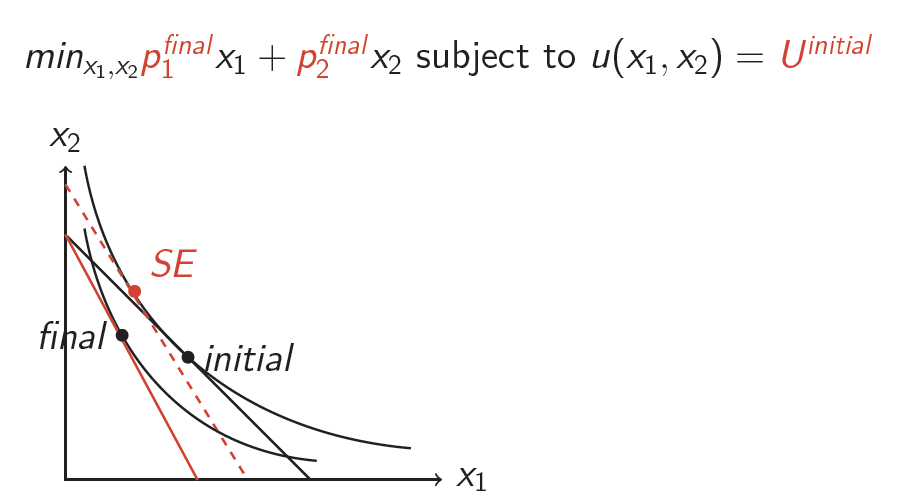
\includegraphics[width=0.8\linewidth]{figure/lec5_1}
				\caption{decomposing total effect into income and substitution effects in graph}
			\end{figure}
			
			\subsubsection{Calculating a Substitution Effect}
				\paragraph{Intuition} to find SE, we need to find the demand of goods with new price level and the origin utility level achieved.
				\begin{multline*}
					\emph{Method: }\\
					\tx{This can be done via expenditure minimization.} \\
					\tx{Let $\overline{U}$ denote the origin utility level.} \\
					\min_{\vec{x}} \vec{p}^{new} \vec{x} + \lambda \times (\overline{U} - u(\vec{x})) \\
					\tx{Extracting the first order conditions: }\\
					\begin{cases}
						\pd{\mc{L}(\cdot)}{x_i} = p_i^{new} - \lambda \pd{u}{x_i} = 0,\ \forall i\\
						\pd{\mc{L}(\cdot)}{\lambda} = \overline{U} - u(\vec{x}) = 0 \\
					\end{cases} \\
					\blacksquare
				\end{multline*}
				and by solving these first order conditions above, we have $h_i(\vec{p}, \overline{U})$ as \textbf{compensated demand curve} (aka Hicksian demand).
		
		\subsection{Income Effect}
			\paragraph{Definition} Income Effect can be captured by proportion of total effect unexplained by substitution effect.
			\[
				\tx{Total Effect} = x_i^{final} - x_i^{initial}
			\]
			\[
				\tx{Substitution Effect} = x_i^{SE} - x_i^{initial}
			\]
			\[
				\tx{Income Effect} = x_i^{final} - x_i^{SE}
			\]
		
		\subsection{Compensated Demand Curve}
			\paragraph{Definition} \textbf{compensated demand curve} captures the changes in quantity demanded for good $i$ when $p_i$ changes, while holding the \underbar{utility} level fixed. And compensated demanded is denoted as
			\[
				h_i(\vec{p}, \overline{U})
			\]
			
			\begin{figure}[h]
				\centering
				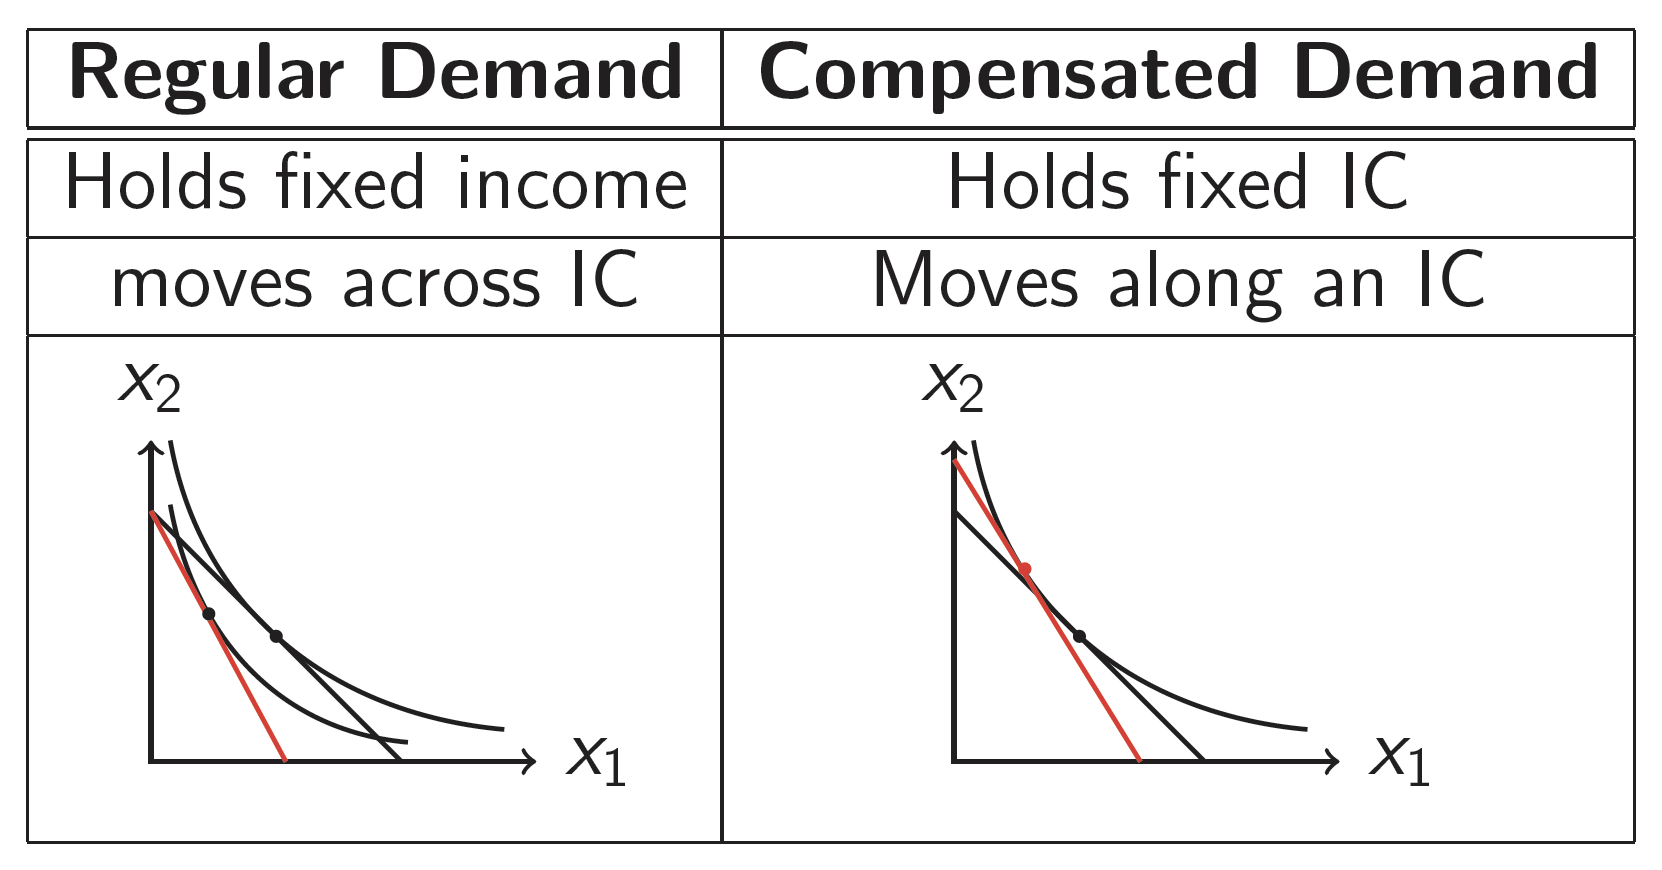
\includegraphics[width=0.7\linewidth]{figure/lec5_2}
				\caption{regular demand and compensated demand on graph: framework 1}
			\end{figure}
			
			\begin{figure}[h]
				\centering
				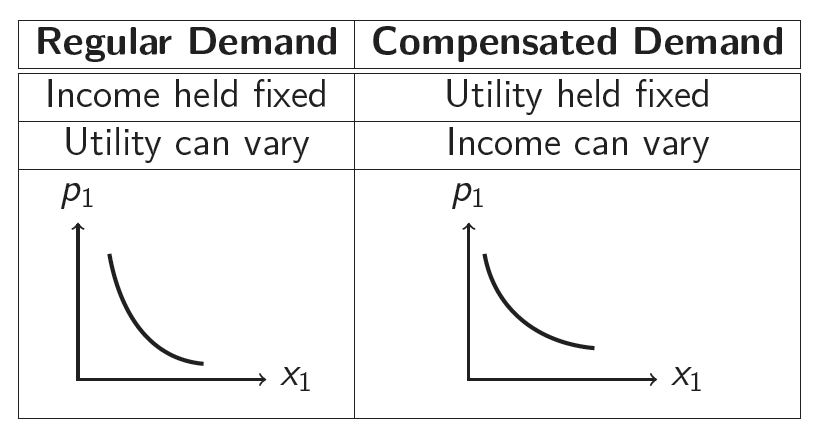
\includegraphics[width=0.7\linewidth]{figure/lec5_3}
				\caption{regular demand and compensated demand on graph: framework 2}
			\end{figure}
		
		\subsection{Slutsky Equation}
			\begin{multline*}
				\emph{Proof.} \\
				h_i(\vec{p}, \overline{U}) = x_i(\vec{p}, I) \\
				\implies h_i(\vec{p}, \overline{U}) = x_i(\vec{p}, e(\vec{p}, \overline{U})) \\
				\implies \pd{h_i}{p_j} = \pd{x_i}{p_j} + \pd{x_i}{I}\pd{E}{p_j} \\
				\implies \pd{h_i}{p_j} = \pd{x_i}{p_j} + \pd{x_i}{I}h_j \\
				\implies \pd{x_i}{p_j} = \pd{h_i}{p_j} - \pd{x_i}{I}h_j \\
				\blacksquare
			\end{multline*}
			
	\section{Lecture 6 Labor Supply and Elasticities}
		\subsection{Model Setup}
			\paragraph{Goods} $c$ \textbf{consumption} and $\ell$ \textbf{leisure}.
			\paragraph{Preference} $u(c, \ell)$.
			\paragraph{Income} \underbar{endogenous} ($L$ \textbf{time endowment}) and \underbar{exogenous} incomes ($M$ as \textbf{non-labor income}).
		
		\subsection{Deriving Labor Supply}
			\[
				\max_{c,\ell} u(c, \ell)\ s.t.\ c + w\ell \leq wL + M
			\]
			By solving the above optimization, we have $(c ^*, \ell ^*)$. And hours of working $h$ is given by $h = L - \ell ^*$.
			
			\subsubsection{Shape of Labor supply}
				\paragraph{Note} notice the assumption on leisure, inferior or normal.
		
\end{document}

































